\documentclass{article}

\usepackage{tikz}
\usepackage{lscape}
\usetikzlibrary{automata, positioning}
\begin{document}
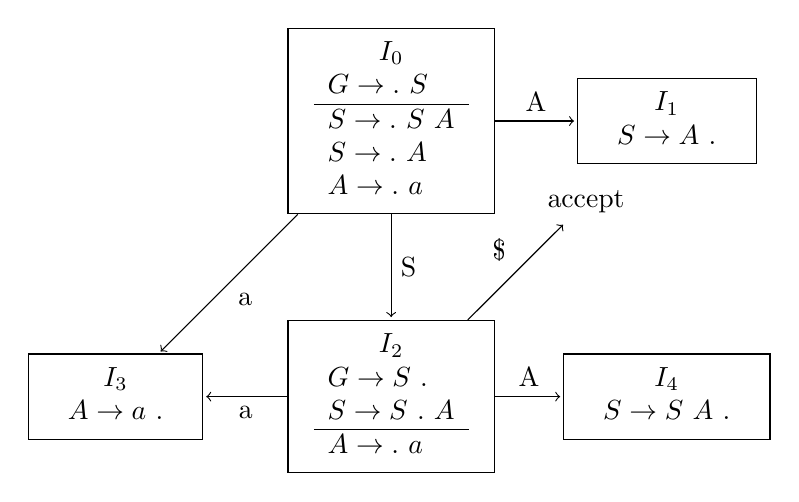
\begin{tikzpicture}[shorten >= 1pt, node distance = 3.5cm, on grid, auto]
  \node[state, rectangle] (0) {
    \begin{tabular}{c} $I_0$ \\
      $\begin{array}{lcl} 
        G \rightarrow .~S \\
        \hline
        S \rightarrow .~S~A \\
        S \rightarrow .~A \\
        A \rightarrow .~a \\
      \end{array}$
    \end{tabular}};
  \node[state, rectangle] [right=of 0] (1) {
    \begin{tabular}{c} $I_1$ \\ 
      $\begin{array}{lcl} 
        S \rightarrow A~. \\
      \end{array}$
    \end{tabular}};
  \node[state, rectangle] [below=of 0] (2) {
    \begin{tabular}{c} $I_2$ \\ 
      $\begin{array}{lcl} 
        G \rightarrow S~. \\
        S \rightarrow S~.~A \\
        \hline
        A \rightarrow .~a \\
      \end{array}$
    \end{tabular}};
  \node[state, rectangle] [right=of 2] (4) {
    \begin{tabular}{c} $I_4$ \\ 
      $\begin{array}{lcl} 
        S \rightarrow S~A~. \\
      \end{array}$
    \end{tabular}};
  \node[state, rectangle] [left=of 2] (3) {
    \begin{tabular}{c} $I_3$ \\ 
      $\begin{array}{lcl} 
        A \rightarrow a~. \\
      \end{array}$
    \end{tabular}};
  \node[] (100) [above right=of 2] {accept};
  \path[->]
    (0) edge node {A} (1)
        edge node {S} (2)
        edge node {a} (3)
    (2) edge node {A} (4)
        edge node {a} (3)
        edge node {\$} (100);
\end{tikzpicture}
\end{document}
